\appendix \chapter{Appendix} 


\section{Deep learning}\label{Annexe:deeplearning}
\subsection{Neural networks}
\subsubsection{A neuron}

Before talking about Convolutional neural network we could ask ourselves what are those neuron we are talking about. In biology the neuron can be represented as in the figure \ref{fig:bioneuron}. The information (input) enter the neuron coming from the dendrites, is processed by the neuron and continues its journey following the axon to the synapses where the connection to an other neuron or group of neurons is made.
\begin{figure}[h!]
   \centerline{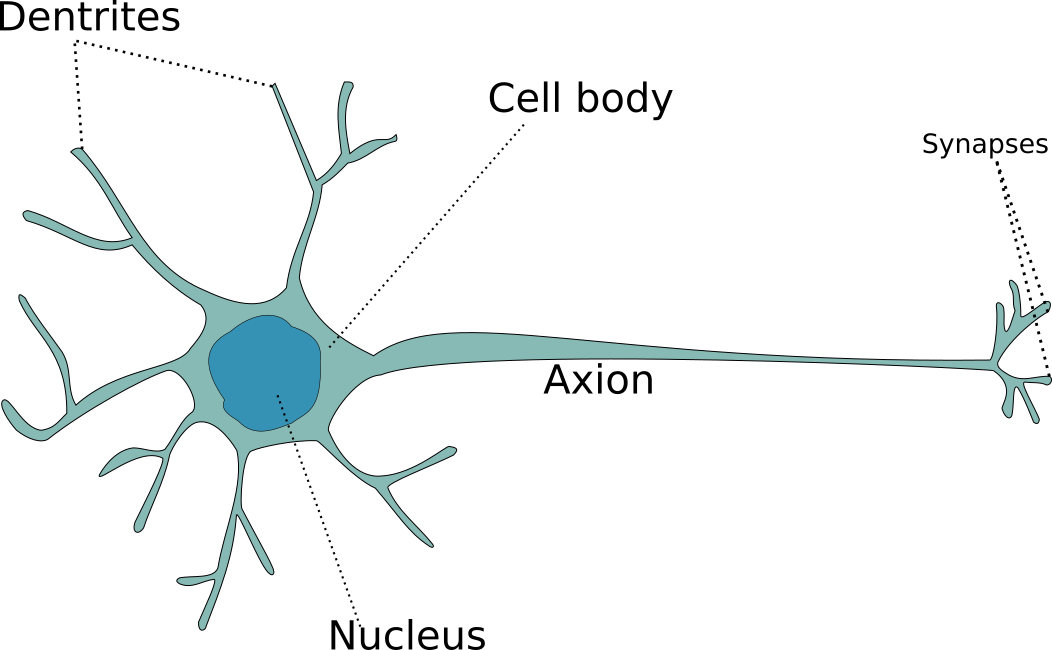
\includegraphics[scale=0.30]{./pics/neuronb.png}}
   \caption{A representation of a biological Neuron}
   \label{fig:bioneuron}
\end{figure}

In machine learning, a neuron is roughly following the same idea. An input is taken processed using a function and an output is given to the next neuron or piece of software. This is represented in figure \ref{fig:artneuron}, several inputs are given to a neuron, with a bias. 

\begin{figure}[h!]
   \centerline{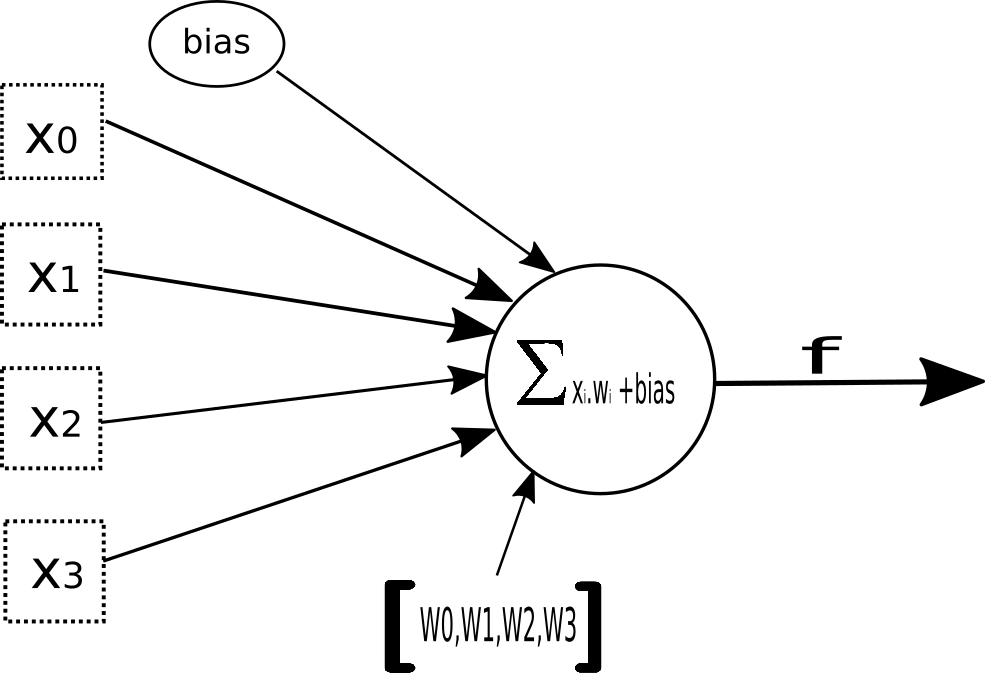
\includegraphics[scale=0.35]{./pics/ArtificialNeuron.png}}
   \caption{A representation of an artificial Neuron }
   \label{fig:artneuron}
\end{figure}

The output of equation \ref{eq:per} is given to an activation function here $f$ given in equation \ref{eq:relu}, which is a RELU function, most commonly used in Convulational neural network nowadays with the sigmoid function represented in equation \ref{eq:sig}. 

\begin{equation}
    y = \sum\limits_{i=1}^n w_ix_i  + bias
    \label{eq:per}
\end{equation}

\begin{equation}
    f(x) = 
 \begin{cases} 
      x & x >0 \\
      0 & otherwise
   \end{cases}
    \label{eq:relu}
\end{equation}

\begin{equation}
    f(x) = \frac{1}{1+ e^{-x}}
    \label{eq:sig}
\end{equation}


This is a basic neuron representation which is the one used in the perceptron algorithm \cite{Rosenblatt58theperceptron} which we are going to see later.

\subsubsection{The Perceptron or premises of modern machine learning}

In 1958 Rosenblatt introduced the perceptron, a probabilistic model modelling in a simpler way the way the brain process information. The goal was to define an algorithm where updatable weights are multiplied by the input to make a decision if the neuron is activated or not. For example for a binary classification problem it would tell us for sample to which class the belongs to, by learning a function separating classes.
The algorithm works as follow for all inputs :
\begin{enumerate}
    \item  Compute the output using the following equation: $x =w_ix_i + bias$ and $output = f(x) = 1 if x >0, -1$ otherwise
    \item Compute gradients : $\Delta w_i = \eta(target - output) x_i$ and $\Delta bias = \eta(target - output)$ ($\eta$ being the learning rate between 0 and 1)
    \item update weights : $w_i = w_i +\Delta w_i$ and $bias = bias + \Delta bias$
\end{enumerate}

In the end, by initializing weights at 0 we can learn a linear function separating our samples as in figure \ref{fig:class}.
\begin{figure}[ht!]
   \centerline{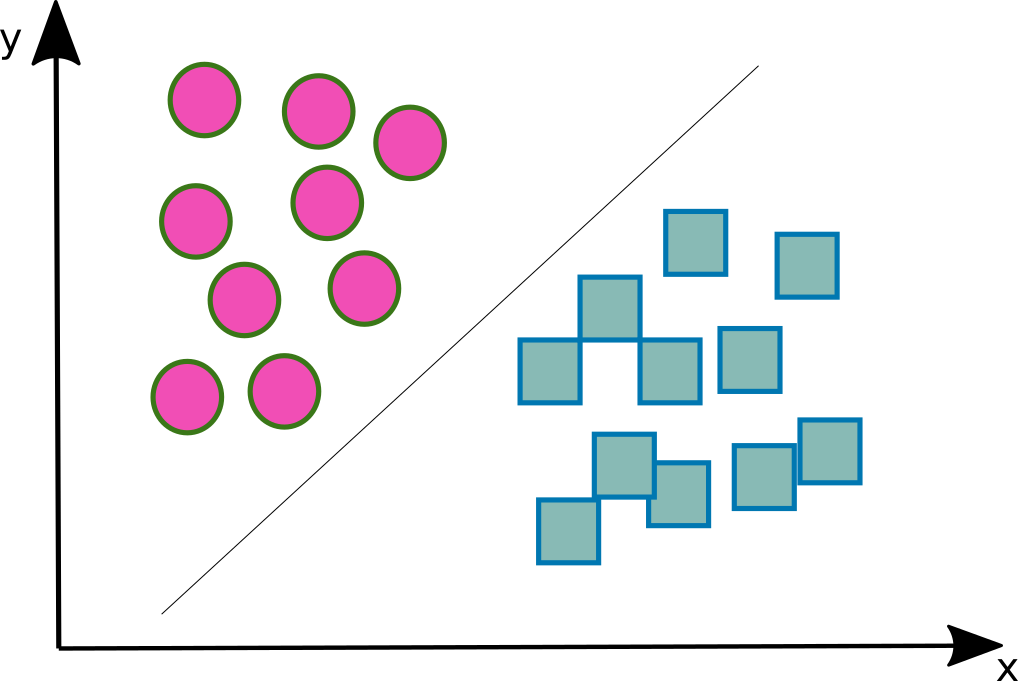
\includegraphics[scale=0.25]{./pics/linear.png}}
   \caption{A binary linear classification of some data}
   \label{fig:class}
\end{figure}

\subsubsection{Multi-layer perceptron/neural network}

A multi-layer perceptron looks as shown in figure \ref{fig:percp}. This is basically multiple neurons connected to each others as "layers". The activation can be a non linear one such as a Sigmoid or piece wise like RELU.
The forward pass (from input to output) is quite straight forward once we define the function $f$. But we also need to update our weights and here comes the idea of back propagation, which can be summed up as, how to learn from our mistakes. The algorithm for a multi-layer perceptron can be summed up as follow:
\begin{enumerate}
    \item Forward the input in the network using the equations we saw previously for each neuron.
    \item Compute the loss between the ouput and the target/ground truth.
    \item Backpropagate the loss in the network updating weights of each neuron.
\end{enumerate}

\begin{figure}[ht!]
   \centerline{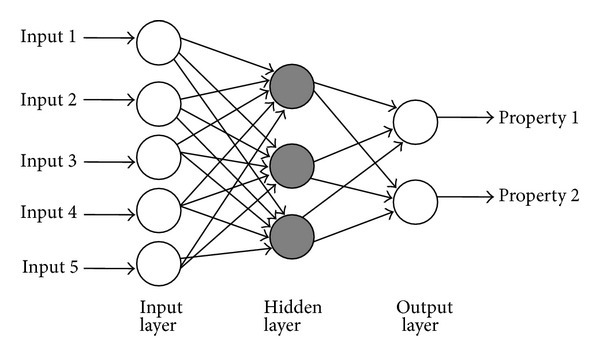
\includegraphics[scale=2.0]{./pics/perceptron.jpeg}}
   \caption{A Multi-layer perceptron (source:cps0715.weebly.com)}
   \label{fig:percp}
\end{figure}

\subsubsection{Loss}

The loss can be obtain using several loss functions depending on the type of output, some famous one we can use are the following:

\textbf{The L1 loss}, which is the mean absolute value of the element-wise difference between input x and target y : $\ell(x, y) = mean(L), L = \{l_1,\dots,l_N\}^\top,  l_n = \left| x_n - y_n \right|$

\textbf{The mean squared error} :  $\ell(x, y) = mean(L), L = \{l_1,\dots,l_N\}^\top,  l_n = \left( x_n - y_n \right)^2 $

or the 


\textbf{Binary Cross Entropy loss } which is : $\ell(x, y) = mean(L) , L = \{l_1,\dots,l_N\}^\top, \\ l_n = \left[ y_n \cdot \log x_n + (1 - y_n) \cdot \log (1 - x_n) \right]$


\subsubsection{Backpropagation}

For the last part we need to execute the backpropagation algorithm. This algorithm can be summed up as , how much each weights impact the output and how to change it to reduce the Total error. Lets take the figure \ref{fig:artneuron} as an example and as an error function the square error $error = \sum\limits_{i=0}^n \frac{1}{2} (y_i - x_i)^2$ (the constant $\frac{1}{2}$ is here to cancel the exponent during differentiation). So applying forward pass we get an Error that we will call $E_{Total}$. Now for the backpropagation part we want to know how much $W_3$ change the $E_{Total}$, which can be written $\frac{ \delta E_{Total}}{\delta W_2}$, the partial derivative of $E_{Total}$ with respect to $W_2$ If we apply the chain rule considering figure \ref{fig:artneuron} we get equation \ref{eq:gradient}.

\begin{equation}
    \frac{ \delta E_{Total}}{\delta W_2} = \frac{ \delta E_{Total}}{\delta outputofneuron}  * \frac{ \delta outputofneuron}{\delta inputofneuron} * \frac{ \delta inputofneuron}{\delta W_2}
    \label{eq:gradient}
\end{equation}
We are going to simply the neuron a bit, by removing inputs to have only two inputs 1 and 2. We have $ E_{Total} = \frac{1}{2} (target - output)^2$ and $\frac{ \delta E_{Total}}{\delta outputofneuron} = 2 * \frac{1}{2} (target - output) * -1 + 0 = -(target - output)  $. Now if we consider that the output of the neuron is computer using sigmoid function \ref{eq:sig}, its partial derivative is $ output ( 1 - output)$. For the result of the neuron function that we call here $inputofneuron$, which is computed as  $ (x_1 * W_1) + (x_2 * W_2) + bias$, its partial derivative would be simply $ x_2$.\\

The calculations above can be summed up as $\frac{ \delta E_{Total}}{\delta W_2} = -(target- output) * output ( 1- output) * x_1 $ and taking $ \delta_2 = \frac{ \delta E_{Total}}{\delta outputofneuron}  * \frac{ \delta outputofneuron}{\delta inputofneuron}$ we get  $  \frac{ \delta E_{Total}}{\delta W_2} \delta_2 * x_2$, which is the usual notation for the "gradient" with respect to $W_2$.\\

Now we need to update the weight $W_2$, which is simply done as : $\textrm{new} W_2 = W_2 + \eta \delta W_2$, with $\eta$ our learning rate.\\

With hidden layers, it becomes a bit more difficult to update weights as they influence output hence error of following layers. This implies taking into consideration the effect of outputs neuron, and making the chain rule a bit more complex, but computation remain the same, and it is not really complicated to implement.
Appendix goes here...